\documentclass{article}
\usepackage{ifthen,algorithmic,amssymb,amsmath,amsthm,verbatim,graphicx, units, tikz,wrapfig, multicol}
\usepackage[top=0.5in, bottom=0.5in, left=0.5in, right=0.5in]{geometry}
\usepackage[utf8]{inputenc}

\pagestyle{empty}
\newboolean{KEY}
% \setboolean{KEY}{true} %prints questions and answers
\setboolean{KEY}{false} %prints questions only
\newcommand{\question}[1]{\ifthenelse{\boolean{KEY}}{}{#1}}
\newcommand{\answer}[1]{\ifthenelse{\boolean{KEY}}{#1}{}}

\newcommand{\eval}[2]{\Bigr| _{#1} ^{#2}}

\begin{document}
\section*{MATH 1215 Practice Final \answer{Key}}
This is a closed-book, closed-notes exam. The only items you are allowed to use are writing implements. If you are caught cheating, you will receive a zero grade for this exam. The max number of points per question is indicated in square brackets after each question. The sum of the max points for all the questions is 61, but note that the max exam score will be capped at 60 (i.e., there is 1 bonus point, but you can't score more than 100\%). You have exactly 60 minutes to complete this exam. Keep your answers clear and concise while complete. Best of luck.

\begin{enumerate}
\item Calculate the arc length of $\ln(\cos x)$ on $[0, \frac{\pi}{4}]$. Simplify. [7]

\answer{
\begin{eqnarray*}
f(x) & = & \ln(\cos x) \\
f'(x) & = & \frac{1}{\cos x}(- \sin x) = - \tan x \\
f'(x)^2 + 1 & = &\tan^2 x + 1 = \sec^2 x \\
\\
L & = & \int _0 ^{\nicefrac{\pi}{4}} \sqrt{1 + f'(x)^2} \ dx \\
  & = & \int _0 ^{\nicefrac{\pi}{4}} \sqrt{\sec^2 x} \ dx \\
  & = & \int _0 ^{\nicefrac{\pi}{4}} \sec x \ dx \\
  & = & \ln | \sec x + \tan x | \eval{0}{\nicefrac{\pi}{4}} \\
  & = & \ln | \sec (\nicefrac{\pi}{4}) + \tan (\nicefrac{\pi}{4})| - \ln | \sec (0) + \tan (0) | \\
  & = & \ln | \sqrt{2} + 1 | - \ln | 1 + 0 | \\
  & = & \ln ( \sqrt{2} + 1)
\end{eqnarray*}
}

\item Calculate the following derivatives:

\begin{enumerate}
  \item $\frac{d^2}{dx^2} (2 \log_7 (x - 3))$ [2]
  \answer{
  \begin{eqnarray*}
    \frac{d}{dx} & = & \frac{2}{(x - 3) \ln 7} \\
    \frac{d^2}{dx^2} & = & \frac{2}{\ln 7} \times \frac{d}{dx} (\frac{1}{x - 3}) \\
                     & = & -\frac{2}{\ln 7 (x - 3)^2}
  \end{eqnarray*}
  }

  \item $\frac{d}{dx} (x^{\sec x})$ [4]
  \answer{
  \begin{eqnarray*}
    x^{\sec x} & = & e ^{\ln x ^{\sec x}} \\
               & = & e ^{\sec x \ln x} \\
    y & = & e ^{\sec x \ln x} \\
    \frac{dy}{dx} & = & e ^{\sec x \ln x} \times \frac{d}{dx} (\sec x \ln x) \\
               & = & e ^{\sec x \ln x} \times (\sec x \tan x (\ln x) + \sec x \frac{1}{x}) \\
               & = & x ^{\sec x} \times (\sec x \tan x (\ln x) + \sec x \frac{1}{x})
  \end{eqnarray*}
  }
\end{enumerate}

\item Classify which function has a faster rate of growth via limit methods \textbf{or} growth classes. If the limits are comparable, identify the growth factor $M$.

\begin{enumerate}
  \item $1.00001^x$ and $x^{40}$. \answer{ $1.00001^x \gg x^{40}$ } [1]
  \item $\ln x^{18}$ and $\ln x$. \answer{ Comparable, $M = 18$ } [1]
  \item  $x \ln x$, $\ln ^3 x$, and $e ^x$. \answer{$\ln ^3 x \gg x \ln x \gg e ^x$} [2]
\end{enumerate}

\item Evaluate the following indefinite integrals, simplification is optional (i.e. $\ln (1), \frac{2}{4}, 5^4$ are all acceptable forms).

\begin{enumerate}
  \item $\int 18x^2 \ln x \ dx$ [4]
  \answer{
  \begin{eqnarray*}
  u = \ln x \quad & & \quad dv = 18x^2 \\
  du = \frac{1}{x} dx \quad & & \quad v = 6x^3
  \\
  \int 18x^2 \ln x \ dx & = & 6x^3 \ln x - \int 6x^2 dx \\
  & = & 6x^3 \ln x - 2x^3 + C
  \end{eqnarray*}
  }

  \item $\int \frac{2}{y^4\sqrt{y^2 - 25}} \ dy$. Assume $\theta$ to be in the first quadrant \emph{at all times}\footnote{Reasoning: this ensures all trigonometric functions will always be positive.}. [8]
  \answer{
  \begin{eqnarray*}
  y & = & 5 \sec \theta \\
  \sqrt{y^2 - 25} & = & \sqrt{25 \sec^2 \theta - 25} \\
  & = & 5\sqrt{\tan^2 \theta} \\
  & = & 5 | \tan \theta | \\
  & = & 5 \tan \theta\\
  \\
  dy & = & 5 \sec \theta \tan \theta \ d\theta \\
  \int \frac{2}{y^4\sqrt{y^2 - 25}} \ dy & = & \int \frac{2}{5^4 \sec^4 \theta (5 \tan \theta)} 5 \sec \theta \tan \theta \ d\theta \\
  & = & \frac{2}{625} \int \frac{1}{\sec^3 \theta} \ d\theta \\
  & = & \frac{2}{625} \int \cos^3 \theta \ d\theta \\
  & = & \frac{2}{625} \int (1 - \sin^2 \theta) \cos \theta \ d\theta \quad u = \sin \theta \\
  & = & \frac{2}{625} \int 1 - u^2 \ du \\
  & = & \frac{2}{625} (u - \frac{1}{3}u^3) + C \\
  & = & \frac{2}{625} (\sin \theta - \frac{1}{3} \sin^3 \theta) + C
  \end{eqnarray*}
  }

  \item $\int \frac{7}{y^2 - 9y - 112} dy$ [5]
  \answer{
  \begin{eqnarray*}
  y^2 - 9y - 112 & = & (y - 16)(y + 7) \\
  \frac{7}{(y - 16)(y + 7)} & = & \frac{A}{y - 16} + \frac{B}{y + 7} \\
  7 & = & A(y + 7) + B(y - 16) \\
  A = \frac{7}{23} & \quad & B = -\frac{7}{23} \\
  \\
  \int \frac{7}{y^2 - 9y - 112} & = & \int \frac{A}{y - 16} + \frac{B}{y + 7} \ dy \\
  & = & \int \frac{\frac{7}{23}}{y - 16} - \frac{\frac{7}{23}}{y + 7} \ dy \\
  & = & \frac{7}{23}(\ln |y - 16| - \ln |y + 7|) + C
  \end{eqnarray*}
  }
\end{enumerate}

\item State the convergence or divergence of the following sequences and series. State all preconditions. Unless specified, use any method.

\begin{enumerate}
  \item $ \{ - \frac{\sin n}{6n} \} $ [3]
  \answer{
  \begin{align*}
  \lim _{n \rightarrow \infty} -\frac{1}{6n} = \lim _{n \rightarrow \infty} \frac{1}{6n} = 0 \\
  -\frac{1}{6n} \ll -\frac{\sin n}{6n} \ll -\frac{1}{6n} \\
  \therefore \text{By Squeeze Theorem, Convergent to 0.}
  \end{align*}
  }

  \item $\sum _{n = 2} ^\infty \frac{1}{1 + n \ln n}$ [5]
  \answer{
  \begin{align*}
  a_n & = \frac{1}{1 + n \ln n} \\
  \text{let } b_n & = \frac{1}{n \ln n} \\
  \\
  \lim _{n \rightarrow \infty} \frac{b_n}{a_n} & = \lim _{n \rightarrow \infty} (1 + \frac{1}{n \ln n}) \\
  & = 1 \\
  \\
  \int _2 ^\infty \frac{dx}{x \ln x} & = \int _2 ^\infty \frac{du}{u} \quad u = \ln x \\
  & = \infty \\
  \therefore \text{By Limit Comparison and} &\  \text{Integral Test, Divergence.}
  \end{align*}
  }

  \item $\sum _{k = 1} ^\infty k \sin (\frac{1}{k})$ [6]
  \answer{
  \begin{eqnarray*}
  \lim _{k \rightarrow \infty} a_k & = & \lim _{k \rightarrow \infty} k \sin(\frac{1}{k}) \\
  & = & \lim \frac{\sin(\frac{1}{k})}{\frac{1}{k}} \\
  & = & \lim \frac{-\frac{\cos(\frac{1}{k})}{k^2}}{-\frac{1}{k^2}} \\
  & = & \cos(\frac{1}{k}) \\
  & = & 1 \\
  & \neq & 0. \\
  \therefore && \text{Diverges by Divergence Test.}
  \end{eqnarray*}
  }
  \end{enumerate}

\begin{multicols}{2}
\item Set up the integral to find the area common to both $r = 2 + \sin \theta$ and $r = 1 - \sin \theta$ as shaded to the right. Do not simplify. \textbf{You do not need to evaluate the integral}. [5]

\answer{
  \begin{equation*}
    \int _{0} ^{2\pi} \frac{1}{2} (2 + \sin \theta)^2 \ d\theta - \int _{-\frac{\pi}{6}} ^{\frac{7\pi}{6}} \frac{1}{2} \left[(2 + \sin \theta)^2 - (1 - \sin \theta)^2 \right]
  \end{equation*}
}

\item Set up the integral to find the pressure experienced by a circular plate with a radius of $2$ that is submerged $6$ meters below the water. This implies that the center of the plate is $8$ meter below the water. Use $\rho$ and $g$ for pressure and acceleration. \textbf{You do not need to evaluate the integral}. [5]
\answer{
  \begin{equation*}
    2 \rho g \int _{-2} ^{2} (8 - y)\sqrt{4 - y^2} \ dy
  \end{equation*}
}

\begin{center}
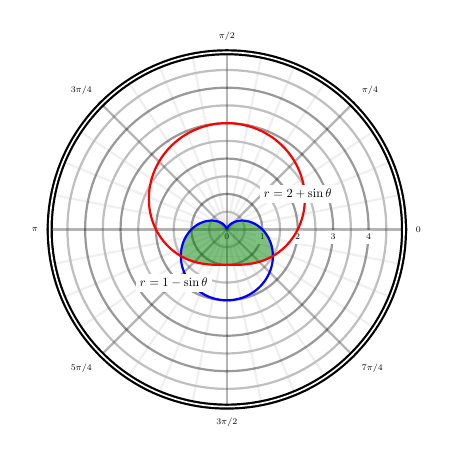
\begin{tikzpicture}[thick,scale=0.45, every node/.style={scale=0.45}]

% Draw the lines at multiples of pi/12
\foreach \ang in {0,...,31} {
  \draw [lightgray,opacity=.25] (0,0) -- (\ang * 180 / 16:5);
}

% Concentric circles and radius labels
\foreach \s in {0, 1, 2, 3, 4} {
  \draw [lightgray] (0,0) circle (\s + 0.5);
  \draw [opacity = .4](0,0) circle (\s);
  \node [fill=white] at (\s, 0) [below] {\scriptsize $\s$};
}

% Add the labels at multiples of pi/4
\foreach \ang/\lab/\dir in {
  0/0/right,
  1/{\pi/4}/{above right},
  2/{\pi/2}/above,
  3/{3\pi/4}/{above left},
  4/{\pi}/left,
  5/{5\pi/4}/{below left},
  7/{7\pi/4}/{below right},
  6/{3\pi/2}/below} {
  \draw [opacity=.25] (0,0) -- (\ang * 180 / 4:5.1);
  \node [fill=white] at (\ang * 180 / 4:5.2) [\dir] {\scriptsize $\lab$};
}

% The double-lined circle around the whole diagram
\draw [style=double] (0,0) circle (5);

\fill [fill=green!50!black, opacity=0.5] plot [domain=-pi/6:7*pi/6] (xy polar cs:angle=\x r,radius= {1-sin(\x r)});

\fill [fill=green!50!black, opacity=0.5] plot [domain=11*pi/6:7*pi/6] (xy polar cs:angle=\x r,radius= {2+sin(\x r)});

\draw [thick,color=blue,domain=0:2*pi,samples=200,smooth] plot (xy polar cs:angle=\x r,radius= {1-sin(\x r)});
\node [fill=white] at (-1.5,-1.5) {$r=1-\sin\theta$};

\draw [thick,color=red,domain=0:2*pi,samples=200,smooth] plot (xy polar cs:angle=\x r,radius= {2+sin(\x r)});
\node [fill=white] at (2,1) {$r=2+\sin\theta$};
\end{tikzpicture}
\end{center}
\end{multicols}

\item Specify your answer as \textit{True} or \textit{False}. No counterexample is need.

\begin{enumerate}
  \item Given $\{ a _n \} ^{\infty} _{n = 1}$, if $a_n$ converges, then it it is bounded. Likewise, if $a_n$ is bounded, then it is convergent. [1] \answer{\textbf{False.}}
  \item If $\{ a_n \}$ and $\{ a_n \}$ are both divergent, then $\{ a_n + b_n \}$ is divergent. [1] \answer{\textbf{False.}}
  \item $\int _0 ^{\pi} \sec \theta \ d\theta$ is an improper integral. [1] \answer{\textbf{True.}}
\end{enumerate}

\end{enumerate}
\end{document}
